\section{Projection}
	In this section we prepare the cube in order to apply the shading algorithm. First we explain how we added textures to the sides of the cube then we explain how we removed the hidden faces.
\subsection{Textures}
In the previous assignment we ended up with a cube drawn as a wireframe and for this first part our task was to map textures in the cube. The faces of the cube are already defined in its own 3D coordinate system and have intuitive names like TopFace, RightFace, etc.\newline

In order to place a texture in each of these faces we created a function with the signature \emph{TextureFace(image, faceVertices, projMethod, imageUrl)}. The parameters this function receives are the current image, the coordinates of the face (faceVertices), the current camera matrix (projMethod) and the url for the texture to be mapped. This function first projects the cube face with the current camera matrix and proceeds to calculate the homography \(H_{C-T}\) between the resulting points and the texture. The resulting homography \(H_{C-T}\) is then used to make the texture mapping with OpenCV's \emph{warpPerspective(...)} function and add the resulting image to the current image with OpenCV's \emph{addWeighted(...)} function.\newline

At this point the result of the texture mapping is correct but the texture looks a bit transparent. To have a better result for the texture mapping we proceed to make a mask by applying a threshold to the result of the \emph{warpPerspective(...)} function and invert it so that the face of the cube is black and the background is white. The mask was then used in a bitwise-and operation with the current image to restore the current background but still have the cube's face in black. After the bitwise-and operation, the result is used in a bitwise-or operation with the colored texture resulting in the correct texture mapping as seen in figure \ref{fig:resultFirstPart}.
\begin{figure}
	\centering
	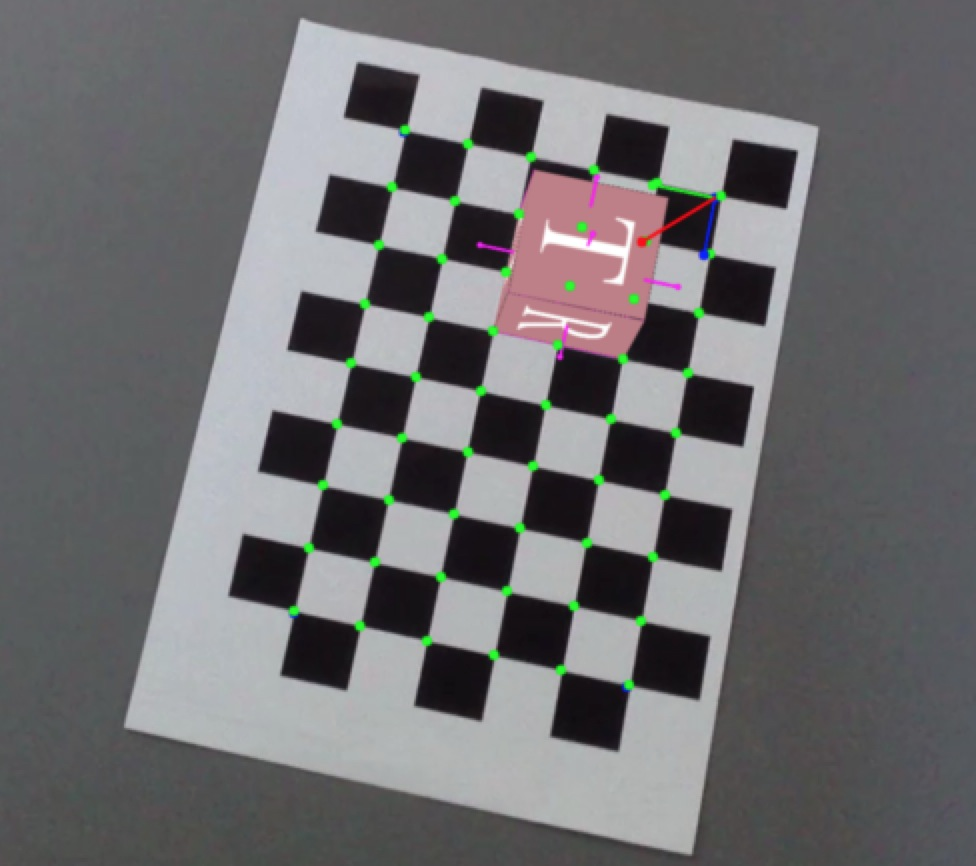
\includegraphics[scale=0.7]{images/textureMapping.jpg}
	\caption{Result of first part. Cube showing mapped textures, calculated normals and hidden faces removed.}
	\label{fig:resultFirstPart}
\end{figure}

\subsection{Back-Face Culling}
After having the textures mapped to the faces of the cube the next task is to remove, or not draw, the hidden faces. For this we first calculate the normals of each face of the unprojected cube. Having calculated the normals the next step is to calculate the vector from the center of the camera, which is done with SIGBTools Camera class. Having the normal vector and the camera center vector we calculate the angle between them. If the angle is greater than 45 degrees the face is removed. The complete result of this first part of the assignment can be seen in figure \ref{fig:resultFirstPart}.